\documentclass[10pt]{article}
\usepackage[letterpaper,margin=1in]{geometry}
\usepackage[T1]{fontenc}
\usepackage{lmodern}
\usepackage{microtype}
\usepackage{amsmath,amssymb}
\usepackage{graphicx}
\usepackage{booktabs}
\usepackage{xcolor}
\usepackage[font=small,labelfont=bf,skip=4pt]{caption}
\usepackage[numbers,sort&compress]{natbib}
\usepackage[colorlinks=true,linkcolor=blue!50!black,citecolor=blue!50!black,urlcolor=blue!50!black]{hyperref}
\setlength{\bibsep}{1pt}
\renewcommand{\arraystretch}{0.95}
\setlength{\textfloatsep}{10pt plus 2pt minus 2pt}

\newcommand{\Ex}{\mathbb{E}}
\newcommand{\pp}{\,\text{pp}}

\title{\vspace{-1.5em}Optimizing Cloud Virtual Machine CPU Reservations via Optimal Policy Trees}
\author{Chris Low \and Emma Li\\[1pt] \small MIT 15.095 Machine Learning under a Modern Optimization Lens, Fall 2026}
\date{\small December 1, 2026}

\begin{document}
\maketitle
\vspace{-1.8em}

\begin{abstract}
\noindent When a virtual machine (VM) is created, a cloud provider must decide how much physical CPU capacity to set aside before the workload is known. We study this decision on 2.47 million VMs from the Azure Public Dataset V2 as a prescriptive problem: each VM receives one of four reservation tiers at a modeled cost that charges for reserved capacity and, with weight $\beta$, for demand above the reservation. Using only creation-time information, an exact depth-3 Optimal Policy Tree with eight leaves lowers modeled cost by 20.1\% relative to the best fixed reservation at $\beta=5$ on the held-out final five days, and a cost-aware Random Forest by 21.6\%. Customer history supplies almost all of this value. Optimizing the decision matters more than predicting utilization well: one forest saves 14.2\% when its predictions are rounded up to a tier and 21.4\% when its leaves are used to estimate the expected cost of each tier. Exact tree optimization improves the training objective but not significantly the test cost relative to greedy trees at $\beta=5$, and a four-leaf exact tree retains 98.6\% of the eight-leaf tree's savings. Savings come from targeting reservations, not reserving less uniformly, and vary widely across customers.
\end{abstract}

\section{Introduction and contributions}
\label{sec:intro}

Many VMs use only a fraction of the CPU they request. Reserving the full request protects performance but idles capacity; reserving less frees capacity but risks contention. The decision is made at creation time, so the question is whether information available then, especially the customer's own history, supports better reservations than a uniform rule. Azure workloads are known to be predictable in this sense \citep{cortez2017resource}.

We ask three questions. (i) Can historical workload information support \emph{interpretable}, cost-aware reservation policies that reduce modeled capacity cost while controlling under-provisioning? (ii) What is gained by optimizing reservation decisions directly instead of minimizing CPU prediction error? (iii) How much do exactly optimized trees add relative to greedy trees and Random Forests, and what is sacrificed in interpretability or robustness?

We apply course methods rather than propose new algorithms. (1) We formulate VM reservation as a four-action prescriptive problem with a fully observed cost matrix and a strictly chronological, leakage-safe evaluation. (2) We solve the Optimal Policy Tree (OPT) problem \citep{amram2022opt} \emph{exactly} over a restricted tree class with a verified dynamic program and compare it with greedy trees, prediction-based rules and a cost-aware Random Forest. (3) We measure the value of customer history, the savings-risk trade-off, the effect of tree size and customer-level outcomes. (4) We implement the two Homework~6 refinements \citep{bertsimas2019mlopt}.

\section{Data and decision problem}
\label{sec:data}

\paragraph{Data and features.} The Azure Public Dataset V2 \citep{azuredataset} records 2,695,548 VMs from one Azure region over 30 days, with subscription (customer), deployment, requested vCPU and memory bucket, creation and deletion times, and summary CPU statistics. We model the 2,468,232 VMs created during the trace. The target $Y_i\in[0,1]$ is the VM's 95th-percentile (P95) CPU utilization as a fraction of its request (test mean 46\%). Each VM has 26 creation-time features: 7 size and time features, 13 subscription-history features and 6 deployment-history features. History statistics (counts, P95 summaries, and shares of past P95 at or below 25/50/75\%) use only VMs of the same subscription or deployment \emph{deleted strictly before} the new VM's creation, since only completed VMs have a known P95. Realized CPU statistics, deletion time, lifetime, the post-hoc \texttt{vmcategory} label and deployment size (which counts future VMs) are never predictors; automated tests enforce this. Missing history is imputed from training rows, with a cold-start flag.

\paragraph{Chronological split.} A training or validation label is usable only if the VM finished before the corresponding cutoff (Table~\ref{tab:split}). This removes 2.5\% of training VMs but 57\% of their vCPU-hours. The test window keeps every VM, including the 4.7\% still running at the end of the trace. Test VMs come almost entirely from repeat customers: 99.9\% belong to subscriptions with at least one completed earlier VM and 91\% to subscriptions with at least 1,000. 69\% of test VMs run for under an hour.

\begin{table}[h]
\centering\small
\caption{Strict chronological split. All tuning uses validation; the test window is used only for evaluation.}
\label{tab:split}
\begin{tabular}{llrr}
\toprule
Split (creation days) & Label rule & VMs & Subscriptions \\
\midrule
Train (0--20) & deleted before day 21 & 1,703,020 & 3,015 \\
Validation (21--24) & deleted before day 25 & 275,143 & 1,462 \\
Test (25--29) & none: all VMs created in the window & 426,846 & 1,726 \\
\bottomrule
\end{tabular}
\end{table}

\paragraph{Decision problem.} Each VM receives a reservation $r\in\mathcal{R}=\{0.25,0.50,0.75,1.00\}$ of its requested CPU at modeled cost
\begin{equation}
C(r,Y;\beta)=r+\beta\max(0,\,Y-r),\qquad \beta>1,
\label{eq:cost}
\end{equation}
which charges for reserved capacity and, with weight $\beta$, for P95 demand above the reservation (the \emph{shortfall}). Because $Y_i$ is observed, every VM has a complete cost vector $C_{ik}=r_k+\beta(Y_i-r_k)^+$, $k=1,\dots,4$, so no counterfactual estimation is needed. A policy $\pi$ maps creation-time features $x$ to a tier and is learned over a class $\Pi$ by
\begin{equation}
\hat\pi\in\arg\min_{\pi\in\Pi}\ \frac{1}{n}\sum_{i=1}^n\sum_{k=1}^4 \mathbb{1}\{\pi(x_i)=r_k\}\,C_{ik}.
\label{eq:erm}
\end{equation}
The objective scores the decision, not an estimate of $Y$. Its pointwise optimum is the tier minimizing $\Ex[C(r,Y;\beta)\mid x]$, which depends on the conditional distribution of $Y$ through $\Ex[(Y-r)^+\mid x]$, not only on its mean. For $\beta\le1$ the answer is always 25\%. We use $\beta=5$ as the main scenario and $\beta=2$ and $10$ as alternatives.

\paragraph{Assumptions.} $\beta$ is an assumed economic trade-off, not an estimated Azure penalty, and the tiers are hypothetical allocation decisions, not observed Azure configurations. We never observe demand or performance under a reduced reservation, so observed P95 utilization serves as a proxy for counterfactual demand. All results therefore concern a \emph{modeled} allocation cost and do not establish Azure billing savings, throttling behavior, physical consolidation savings or SLA compliance.

\section{Methodology}
\label{sec:methods}

\paragraph{Benchmarks.} The \emph{best fixed} rule applies the tier with the lowest validation cost to every VM (50\% at $\beta=2$, 100\% at $\beta=5,10$); all savings are relative to it. A transparent customer rule, H1, rounds the subscription's mean past P95 plus a validation-tuned margin up to a tier. The hindsight \emph{oracle} gives each VM its cost-minimizing tier using the realized $Y_i$; it is infeasible and serves only as a bound.

\paragraph{Prediction-based rules.} Ridge regression, CART (32 leaves, chosen on validation) and a Random Forest (RF; 100 trees, minimum leaf 50) \citep{breiman2001rf} predict P95 from all 26 features. A prediction $\hat y$ becomes a decision by rounding up to the smallest tier $\ge\hat y$, or by rounding up $\hat y+\delta$ with a margin $\delta$ tuned on validation for each $\beta$. This is the predict-then-optimize pattern studied by \citet{elmachtoub2022spo}.

\paragraph{Cost-aware Random Forest.} A multi-output RF with the same settings predicts the shortfalls $\big((Y-0.25)^+,(Y-0.5)^+,(Y-0.75)^+\big)$, estimating $\Ex[(Y-r_k)^+\mid x]$, and chooses $\arg\min_k r_k+\beta\,\widehat{\Ex}[(Y-r_k)^+\mid x]$.

\paragraph{Greedy policy trees.} Trees use 8 features chosen by validation permutation importance of the cost-aware RF at $\beta=5$: the subscription's mean and median past P95, its shares of past VMs with P95 $\le75\%$ and $\le50\%$, vCPU bucket, memory bucket, memory per vCPU and the deployment's mean past P95. Each feature is cut into at most 32 training-quantile bins, which gives every tree method the same 31 candidate thresholds per feature. The greedy tree chooses each split top-down to minimize the cost \eqref{eq:erm} of its two children. Depth (1--3) and minimum leaf size (0.1--5\% of training VMs) are chosen on validation for each $\beta$.

\subsection{Exact Optimal Policy Trees}
\label{sec:opt}

Optimal Policy Trees \citep{amram2022opt}, \citep[Ch.~14]{bertsimas2019mlopt} minimize \eqref{eq:erm} over trees of bounded depth; the commercial implementation does so by local search. Our tree class is finite, so we solve the problem exactly.

\paragraph{Tree class.} $\Pi_{D,m}$ contains every tree of depth at most $D$ whose internal nodes test $x_j\le\theta$ for one of the 8 features $j$ and one of its 31 candidate thresholds $\theta$, whose leaves each contain at least $m$ training VMs, and whose leaves may take any of the four tiers. Shallower trees belong to the class.

\paragraph{Recursion.} Let $R$ be a region of feature space reached by a path of splits. The best cost achievable in $R$ with at most $d$ further levels is
\begin{equation}
V_d(R)=\min\Big\{\textstyle\min_k \sum_{i\in R}C_{ik}\ \ (\text{if }|R|\ge m),\ \ \min_{j,\theta}\big[V_{d-1}(R\cap\{x_j\le\theta\})+V_{d-1}(R\cap\{x_j>\theta\})\big]\Big\},
\label{eq:dp}
\end{equation}
where $V_0(R)$ is the best single-tier leaf cost (infinite if $|R|<m$). $V_D(\text{all data})$ is the optimal training cost and the minimizing choices define the tree.

\paragraph{Why it is tractable.} Two facts make complete enumeration of \eqref{eq:dp} fast. First, the cost of any leaf, for any tier and any $\beta$, is linear in four sufficient statistics: $\sum_{i\in L}C_{ik}=n_Lr_k+\beta S_{L,k}$, with $n_L$ the count and $S_{L,k}=\sum_{i\in L}(Y_i-r_k)^+$. Second, after discretization the 1.70 million training VMs collapse to 46,673 distinct feature patterns, each carrying its own statistics. For depth 3 we enumerate every root split; below it, for each pair of features used at the second and third levels, a three-dimensional histogram of the statistics with two-dimensional prefix sums gives the cost of every grandchild region for all threshold pairs at once. One depth-3 tree takes about 5 seconds and the full validation grid about a minute. Depth 4, a root split followed by an exact depth-3 search in each child, takes 28--36 minutes.

\paragraph{What is certified.} Because \eqref{eq:dp} is evaluated over every allowed split, the returned tree is a global minimizer of \emph{training} cost within $\Pi_{D,m}$. This is a statement about one finite class: it does not cover continuous thresholds, features outside the eight, deeper trees, or test performance.

\paragraph{Verification.} The solver matches brute-force enumeration at depths 2 and 3. Against an independent Gurobi mixed-integer formulation on 1,000 and 5,000 VMs, Gurobi proved the same depth-2 optimum in 86 and 212 seconds (the DP takes milliseconds), and at depth 3 stopped at its 600-second limit with 7.5--13.1\% gaps without finding a better tree. Interpretable AI's local search \citep{iai} reached the optimum in 3 of 4 such checks but failed on the full training set. \texttt{policytree} \citep{sverdrup2020policytree} also searches discretized thresholds exhaustively.

\paragraph{Evaluation.} Every selection (tiers, margins, depth, leaf sizes, cluster count) uses validation data. On the test window we report mean modeled cost, saving relative to best fixed, mean reservation $\Ex[r]$, exceedance frequency $P(Y>r)$, expected shortfall $\Ex[(Y-r)^+]$ in percentage points (pp) of VM capacity, and severe shortfall $P(Y-r>20\pp)$. 95\% intervals come from a paired bootstrap over the 1,726 test subscriptions (1,000 replicates); they treat trained policies as fixed, are not adjusted for multiple comparisons, and when they contain zero they show no significant difference, not equivalence.

\section{Main experimental results}
\label{sec:results}

\begin{table}[t]
\centering\small
\caption{Test results. Columns 2--7 at $\beta=5$, where the validation-selected best fixed tier is 100\%; savings are relative to the best fixed tier at each $\beta$. $\Ex[r]$ in \% of capacity, shortfall in pp.}
\label{tab:main}
\setlength{\tabcolsep}{4pt}
\begin{tabular}{lrrrrrr|rr}
\toprule
 & \multicolumn{6}{c|}{$\beta=5$} & \multicolumn{2}{c}{\% saving} \\
Policy & Cost & \% saving & $\Ex[r]$ & $P(Y{>}r)$ & $\Ex[(Y{-}r)^+]$ & $P(Y{-}r{>}20)$ & $\beta{=}2$ & $\beta{=}10$ \\
\midrule
Best fixed tier (validation) & 1.000 & 0.0 & 100.0 & 0.0 & 0.00 & 0.0 & 0.0 & 0.0 \\
H1: customer mean P95 + margin & 0.809 & 19.1 & 72.5 & 11.7 & 1.67 & 3.5 & 11.3 & 14.3 \\
RF prediction, rounded up & 0.858 & 14.2 & 59.0 & 29.9 & 5.35 & 13.1 & 11.7 & $-$12.5 \\
RF prediction + margin & 0.802 & 19.8 & 73.2 & 10.0 & 1.41 & 2.8 & 12.4 & 15.3 \\
Greedy policy tree (5 leaves) & 0.800 & 20.0 & 74.3 & 8.1 & 1.14 & 2.3 & 11.4 & 14.8 \\
\textbf{Exact OPT, depth 3 (8 leaves)} & \textbf{0.799} & \textbf{20.1} & 73.4 & 9.3 & 1.30 & 2.6 & 11.5 & 15.3 \\
Cost-aware RF & 0.784 & 21.6 & 72.5 & 9.1 & 1.18 & 2.2 & 12.9 & 16.7 \\
Forest-weighted prescription (\S\ref{sec:refine}) & 0.786 & 21.4 & 72.5 & 9.2 & 1.22 & 2.2 & 13.2 & 16.5 \\
\midrule
Oracle (hindsight, infeasible) & 0.589 & 41.1 & 57.7 & 9.9 & 0.25 & 0.0 & 27.7 & 40.5 \\
\bottomrule
\end{tabular}
\end{table}

\paragraph{Benchmark.} Table~\ref{tab:main} compares the policies. OPT's 20.1\% saving at $\beta=5$ has a subscription-clustered interval of [14.1\%, 26.9\%], wide because a few large customers dominate the trace; paired differences between policies are much tighter. OPT is cheaper than the customer rule H1 by 0.0095 [0.0041, 0.0163] at $\beta=5$, and costlier than the cost-aware RF at every $\beta$ (by 0.0112, 0.0149 and 0.0141 at $\beta=2,5,10$, all intervals excluding zero). The tree therefore keeps 89--93\% of the RF's savings. Weighting by vCPUs or vCPU-hours lowers savings by 1--5 points without changing the ordering.

\begin{figure}[t]
\centering
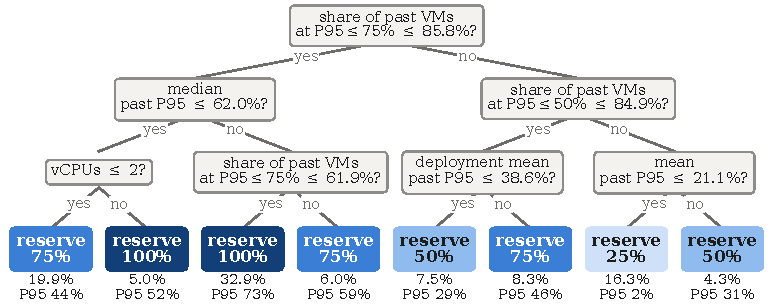
\includegraphics[width=\textwidth]{figures/fig_opt_tree.pdf}
\caption{Exact depth-3 OPT at $\beta=5$, trained on 1.70M VMs; it minimizes training cost over the restricted class $\Pi_{3,m}$. All splits except ``vCPUs'' and ``deployment mean'' use the \emph{customer's} (subscription's) completed VMs. Below each leaf: share of test VMs and their mean realized P95.}
\label{fig:tree}
\end{figure}

\paragraph{The learned policy.} The $\beta=5$ tree (Figure~\ref{fig:tree}) first asks how often the customer's past VMs exceeded 75\% P95, an upper-tail question rather than an average. Near-idle customers (16.3\% of test VMs, mean realized P95 of 2\%) receive 25\%; customers with frequent hot VMs keep 100\% unless their VMs are small.

\paragraph{Customer history is the dominant source of value.} A nested feature ablation (Figure~\ref{fig:ablation}) retrains each method on three feature sets. With size and creation time alone, OPT saves 6.0\% at $\beta=5$ and 0.9\% at $\beta=10$; adding subscription history raises these to 20.3\% and 15.1\%, and deployment history then changes little. VM size and arrival time say little about how hard a VM will run, whereas a customer's past VMs are a direct sample of the same workload distribution, and the upper tail of that sample is exactly what the reservation decision needs. The choice of method adds at most about 1.5 points on top of this information.

\begin{figure}[t]
\centering
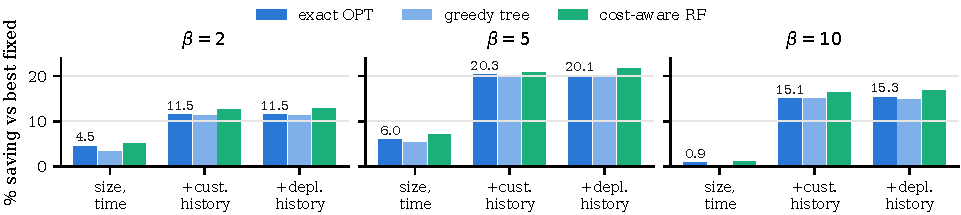
\includegraphics[width=\textwidth]{figures/fig_ablation.pdf}
\caption{Feature ablation: test saving relative to best fixed when each method is retrained on nested feature sets. Labels give exact OPT's saving.}
\label{fig:ablation}
\end{figure}

\paragraph{Prediction accuracy versus decision quality.} The RF predicts P95 better than Ridge and CART (test $R^2$ of 0.525 versus 0.494 and 0.491), yet its root mean squared error of 25.0\pp{} equals one tier width and one VM in six is under-predicted by more than 25\pp. Rounding these unbiased predictions up leaves 29.9\% of VMs under-provisioned and is worse than the fixed rule for $\beta\ge8$. A tuned margin repairs much of this, and the three regressors with margins then differ by at most 2.2 points, not in the order of their $R^2$. With this forest fixed, the decision rule matters more than accuracy: cost at $\beta=5$ falls from 0.858 (round up) to 0.802 (margin) to 0.786 (forest-weighted, \S\ref{sec:refine}).

\paragraph{Why exact OPT barely beats greedy.} Exact optimization lowers \emph{training} cost by 0.4--0.5\% relative to the greedy tree at each $\beta$, as it must. On test, OPT minus greedy is $-0.0012$ [$-0.0058$, 0.0040] at $\beta=2$ and $-0.0013$ [$-0.0054$, 0.0027] at $\beta=5$, neither significant, and $-0.0057$ [$-0.0110$, $-0.0014$] at $\beta=10$. A training gain this small is within the drift between periods and does not reliably carry over. Greedy also has little to lose here: one strongly informative variable family, the customer's past P95 distribution, dominates the first splits, so a myopic choice is rarely a trap. Exactness does buy stability: from 200,000 training VMs upward the exact tree is identical across five random samples, unlike local-search OPT.

\paragraph{How the forest improves on the tree.} The cost-aware RF is 1.6--1.9\% cheaper than OPT. Most of the gap is flexibility rather than information: restricted to the tree's 8 features, the RF still costs 0.787 at $\beta=5$, against 0.799 for OPT. A hundred deep trees can separate customers that an eight-leaf partition must treat alike, at the price of a policy no one can inspect.

\paragraph{Targeting, not uniform reduction.} At $\beta=5$, OPT reserves 26.6 points less than the fixed rule and pays a shortfall penalty of 6.5 points of cost. Assigning OPT's own tier mix to VMs \emph{at random} would raise expected shortfall from 1.30\pp{} to 8.0\pp{} and cost 13.4\% \emph{more} than always reserving 100\%. Equivalently, a randomized fixed-tier rule with OPT's expected shortfall must reserve 93\% of capacity, against OPT's 73\% (Figure~\ref{fig:beta}b). The counterfactual separates two explanations of the savings, reserving less and reserving \emph{well}, and shows that all of the gain comes from the second.

\paragraph{Beyond cost.} At $\beta=5$ every learned policy except rounded-up prediction exceeds its reservation on 8--12\% of VMs, with expected shortfall of 1.1--1.7\pp{} and 2.2--3.5\% of VMs short by more than 20\pp{} (Table~\ref{tab:main}). Lower cost does not imply fewer exceedances: greedy exceeds less often than OPT but reserves more, while the cost-aware RF reserves less with no more exceedance.

\section{Refinements from the book}
\label{sec:refine}

Homework~6 Question~2(b) selected suggestion \#7, interpretable clustering \citep[Ch.~20, \S\S20.1--20.2]{bertsimas2019mlopt}, and suggestion \#10, distribution-aware prescription \citep[Ch.~13, \S\S13.1--13.2]{bertsimas2019mlopt}. Both use the strict split with every choice made on validation and are compared with the fixed tier, OPT and the cost-aware RF on cost, reservation and shortfall (Table~\ref{tab:refine}).

\begin{table}[t]
\centering\small
\caption{Refinements from the book (test). Rules A--C use one identical P95 forest. For reference, OPT costs 0.699 / 0.799 / 0.847 and the cost-aware RF 0.687 / 0.784 / 0.833 at $\beta=2/5/10$.}
\label{tab:refine}
\setlength{\tabcolsep}{5pt}
\begin{tabular}{lrrr|rrr}
\toprule
 & \multicolumn{3}{c|}{Test cost} & \multicolumn{3}{c}{$\beta=5$} \\
Policy & $\beta{=}2$ & $\beta{=}5$ & $\beta{=}10$ & \% saving & $\Ex[r]$ & $\Ex[(Y{-}r)^+]$ \\
\midrule
k-means ($K=8$) $\to$ tier per cluster & 0.703 & 0.803 & 0.870 & 19.7 & 72.9 & 1.49 \\
OCT (depth 4) $\to$ cluster $\to$ tier & 0.701 & 0.805 & 0.869 & 19.5 & 74.0 & 1.30 \\
\midrule
A: point prediction, rounded up & 0.697 & 0.858 & 1.125 & 14.2 & 59.0 & 5.35 \\
B: point prediction + margin & 0.692 & 0.802 & 0.847 & 19.8 & 73.2 & 1.41 \\
C: forest-weighted prescription & 0.685 & 0.786 & 0.835 & 21.4 & 72.5 & 1.22 \\
\bottomrule
\end{tabular}
\end{table}

\subsection{Refinement 1: Interpretable clustering (Chapter 20, Sections 20.1--20.2)}

Following \S20.1 we ran k-means \citep{lloyd1982kmeans} on eight standardized creation-time features (log vCPU and memory, the customer's mean and median past P95 and shares of past VMs above 75\% and 50\%, log count of completed customer VMs, and the deployment's mean past P95), fitting the scaler and centroids on training rows; validation cost at $\beta=5$ selected $K=8$. Each cluster receives the tier with the lowest \emph{training} cost for each $\beta$, so the clusters come from feature similarity and only the tier assignment uses the cost. Following \S20.2 \citep{bertsimas2017oct,bertsimas2021clustering}, a depth-4 Optimal Classification Tree reproduces the cluster labels from the raw features, giving readable routing rules. The clusters order by the customer's past P95 level and upper tail; at $\beta=5$ a near-idle group (15\% of VMs) receives 25\% and four groups receive 100\%. The OCT agrees with k-means on 88.9\% of test VMs and changes cost by only 0.0015. Clustering saves 19.7\% at $\beta=5$, against 20.1\% for OPT and 21.6\% for the cost-aware RF; the difference from OPT is not statistically significant ($+0.0044$ [$-0.0047$, 0.0140]). At $\beta=10$ it falls clearly behind OPT (13.0\% versus 15.3\%; $+0.0228$ [0.0103, 0.0365]): costly errors then concentrate among customers with a heavy upper tail, which OPT isolates with a threshold on the share of past VMs above 75\%, while similarity-based clusters ignore that boundary and under-provision more VMs (4.5\% versus 3.4\%). Clustering describes the customer population well but does not replace optimizing the cost.

\subsection{Refinement 2: Distribution-aware prescriptive optimization (Chapter 13, Sections 13.1--13.2)}

Section 13.1 casts the decision as minimizing conditional expected cost, estimated in \S13.2 by weighting training observations \citep{bertsimas2020predictive}. With the main P95 forest $\{L_t\}_{t=1}^{100}$, training VM $i$ receives the weight of the leaves it shares with a new VM $x$, as in quantile regression forests \citep{meinshausen2006qrf}, and $x$ receives the cheapest tier under the weighted cost:
\begin{equation}
\hat r(x)\in\arg\min_{r\in\mathcal{R}}\ \sum_{i=1}^{n} w_i(x)\big[r+\beta\,(Y_i-r)^+\big],\qquad
w_i(x)=\frac{1}{100}\sum_{t=1}^{100}\frac{\mathbb{1}\{x_i\in L_t(x)\}}{|L_t(x)|}.
\label{eq:forest}
\end{equation}
On this one forest we compare (A) rounding the point prediction up, (B) adding a validation-tuned margin first, and (C) solving \eqref{eq:forest}. At $\beta=5$ cost falls from 0.858 (A) to 0.802 (B) and 0.786 (C). C is cheaper than B at every $\beta$ (by 0.0167 [0.0117, 0.0230] at $\beta=5$; at $\beta=10$ the interval only just excludes zero), reserves less (72.5\% versus 73.2\%) with lower expected shortfall (1.22 versus 1.41\pp), and is not significantly different from the separately trained cost-aware RF. B shifts every prediction by one margin; C responds to the shape of each VM's conditional demand. VMs predicted at 40--50\% (24\% of the test window) have realized P95 spanning all four tiers: rounding up gives them all 50\% and leaves 41\% exceeded, while C raises the tier where the weighted neighbors run hot and lowers it where they are idle, leaving 16\% exceeded. Predicting mean utilization accurately is not the same as choosing the reservation that minimizes expected cost.

\section{Sensitivity, complexity and robustness}
\label{sec:robust}


\paragraph{Economic sensitivity.} Every method was re-tuned on validation at 12 values of $\beta$ from 1.5 to 20 (Figure~\ref{fig:beta}a); costs at different $\beta$ are never compared to choose $\beta$. OPT's saving rises from 5.2\% at $\beta=1.5$ to 20.1\% at 5 and declines to 15.3\% at 10 and 13.3\% at 20. The peak near 5 occurs because the validation-selected fixed tier jumps from 75\% to 100\% at $\beta=4.46$, so just above that point the uniform baseline is most wasteful. (Against the test-hindsight 75\% tier, OPT's $\beta=5$ saving is 19.6\%.) The broad ordering is stable across the grid: the forest-based rules lead, the trees follow closely, rounded-up prediction collapses at high $\beta$, and the cost-aware RF is significantly cheaper than OPT at all 12 values. The $\beta=5$ tree tolerates a misjudged penalty: for a true $\beta$ in $[4,8]$ it costs under 1\% more on test than a tree re-optimized for that value (2--3\% at 3 or 10, 15--17\% at 1.5 or 20).

\begin{figure}[t]
\centering
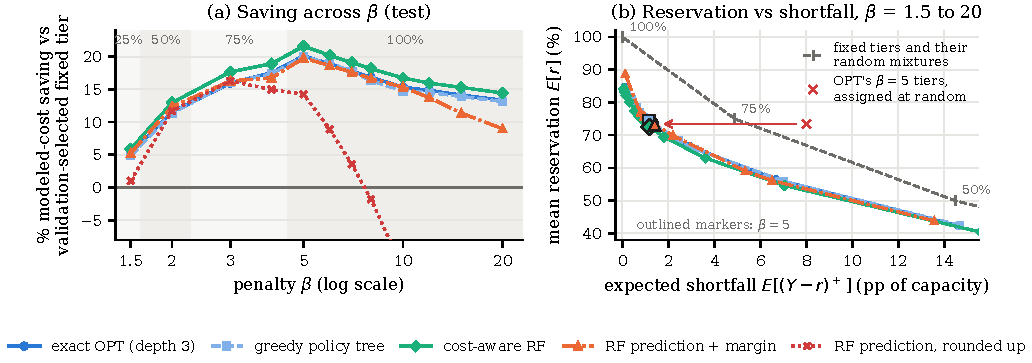
\includegraphics[width=\textwidth]{figures/fig_beta_risk.pdf}
\caption{(a) Test saving relative to the validation-selected best fixed tier at 12 values of $\beta$, with every policy re-tuned on validation at each $\beta$. Shaded bands mark the best fixed tier chosen on validation. The forest-weighted prescription (not shown) tracks the cost-aware RF. (b) Mean reservation versus expected shortfall of the same configurations; lower left is better. Dashed: fixed tiers and their random mixtures. Red cross: OPT's $\beta=5$ tier mix assigned to VMs at random.}
\label{fig:beta}
\end{figure}

\begin{table}[t]
\centering\small
\caption{Complexity and customer-level outcomes at $\beta=5$ (test). $\Delta$: paired cost difference to depth-3 OPT with 95\% subscription-clustered interval. Equal-subscription columns weight each of the 1,036 subscriptions with $\ge5$ test VMs equally (exploratory).}
\label{tab:complex}
\setlength{\tabcolsep}{4pt}
\begin{tabular}{lrrlrr|rr}
\toprule
 & & & & & & \multicolumn{2}{c}{Equal-subscription} \\
Policy & Leaves & Cost & $\Delta$ vs depth-3 OPT [95\% CI] & $\Ex[r]$ & $P(Y{>}r)$ & \% saving & $P(Y{>}r)$ \\
\midrule
Exact OPT, depth 2 & 4 & 0.802 & $+0.0028$ [$-0.0017$, 0.0079] & 74.6 & 7.7 & 18.2 & 11.2 \\
Exact OPT, leaf-penalized & 5 & 0.796 & $-0.0029$ [$-0.0101$, 0.0027] & 73.5 & 8.6 & 18.5 & 11.7 \\
\textbf{Exact OPT, depth 3} & 8 & 0.799 & -- & 73.4 & 9.3 & 17.6 & 13.1 \\
Exact OPT, depth 4 & 16 & 0.795 & $-0.0040$ [$-0.0088$, 0.0002] & 73.8 & 8.4 & 18.1 & 12.4 \\
Greedy policy tree & 5 & 0.800 & $+0.0013$ [$-0.0027$, 0.0054] & 74.3 & 8.1 & 18.3 & 11.4 \\
Cost-aware RF & -- & 0.784 & $-0.0149$ [$-0.0238$, $-0.0069$] & 72.5 & 9.1 & 18.9 & 10.3 \\
\bottomrule
\end{tabular}
\end{table}

\paragraph{Tree complexity and interpretability.} Table~\ref{tab:complex} compares exact trees of different sizes. Besides the main depth-3 model, each variant is chosen by its own validation rule (the five-leaf tree is the simplest within 0.1\% of the best validation cost along an exact per-leaf penalty path). A four-leaf tree keeps 98.6\% of the eight-leaf tree's savings at $\beta=5$ and 94--100\% across all 12 values of $\beta$; its cost differences from the eight-leaf tree are not significant at $\beta=2,5,10$ (which does not establish equivalence). Depth 4 doubles the leaves for 0.5--1.0\% lower test cost, significant only at $\beta=2$ and 10, and at $\beta=10$ it gains by reserving 1.5 points less while exceedance rises from 3.4\% to 4.6\%. Operationally, a four-leaf rule is two questions about a customer's history that an operator can audit, explain and re-derive when the fleet changes; a 16-leaf tree or a 100-tree forest cannot be checked that way, and the cost-aware RF's further 1.5 points are the price of giving that up.

\paragraph{Operational risk.} The objective penalizes the \emph{magnitude} of shortfall, not its frequency. Even the oracle exceeds on 9.9\% of VMs at $\beta=5$, because a small overshoot is cheaper than the next tier; the learned policies differ in severity. When OPT under-reserves, the shortfall averages 14\pp{} (oracle 2.5\pp), with a 95th percentile of 36.7\pp{} (cost-aware RF 28.6\pp); about 80\% of these VMs have realized P95 above 75\%. Two-tier under-reservation is rare (0.7\% of VMs); 19\% of VMs remain two or more tiers above need. At $\beta=2$ the cost-aware RF's lower cost comes with 2.3 points more exceedance than OPT.

\paragraph{Customer heterogeneity.} The objective weights each VM equally, so a customer with 40,000 VMs counts 10,000 times as much as one with four, and aggregate savings describe large customers best. At $\beta=5$ the median subscription with at least 5 test VMs saves 10.4\% under OPT, about half the aggregate 20.1\%. The 94 subscriptions with at least 1,000 test VMs hold 78\% of VMs and 85\% of OPT's saving. Under OPT, 11.9\% of subscriptions pay more than under always-100\% (7.6--7.7\% for greedy, four-leaf and RF). Weighting subscriptions equally (Table~\ref{tab:complex}) reverses the order of the trees: the eight-leaf OPT has the lowest saving and the highest exceedance, and greedy, the four-leaf tree and the RF are cheaper per subscription by 0.006--0.013 with intervals excluding zero. Validation shows the same pattern, consistent with the extra leaves fitting a cost dominated by large customers. The analysis is exploratory, not a fairness objective.

\section{Limitations and conclusion}
\label{sec:conclusion}

\paragraph{Limitations.} All savings are modeled. $\beta$ is assumed, the tiers are hypothetical, and we never observe demand or performance under a reduced reservation, so we make no claim about Azure billing, throttling, consolidation or SLA compliance. The optimality certificate covers training cost within $\Pi_{D,m}$ only. The data cover one region and 30 days with a five-day test window; P95 values of short-lived VMs rest on few readings, and the label rule removes most long-lived training VMs. Features were selected once at $\beta=5$, validation selection is noisy, and the bootstrap intervals hold policies fixed without multiplicity adjustment.

\paragraph{Conclusion.} Historical customer utilization supports interpretable reservation policies that cut modeled capacity cost by about 20\% at $\beta=5$ and 15--20\% for $\beta\in[3,10]$. At $\beta=5$, about 9\% of VMs exceed their reservation, by 14\pp{} on average, and 2--3\% by more than 20\pp. The gains come from matching reservations to workloads and require learning from the cost, not from prediction error. Exact optimization makes OPT certifiable, fast and stable, but it gains little over greedy trees on test, a four-leaf tree performs comparably, and a cost-aware forest is about 1.5 points cheaper. Deployment would require a shadow trial with enforced reservations, a $\beta$ calibrated from service-level costs, and monitoring of customer-level outcomes.

{\footnotesize
\bibliographystyle{abbrvnat}
\bibliography{references}
}

\end{document}
